\documentclass[a4paper, 14pt]{extarticle}
\usepackage[top=1in, bottom=1in, left=1in, right=1in]{geometry}
\usepackage{amsmath}
\usepackage{amssymb}
\usepackage{graphicx}
\usepackage{hyperref}
\usepackage{tcolorbox}
\usepackage{tikz}
\usepackage{tikz-3dplot}
\usepackage{enumitem}
\usepackage{fontspec}
%\usetikzlibrary{decorations.pathmorphing}
\usetikzlibrary{calc,decorations,patterns,arrows,decorations.pathmorphing,3d}
\definecolor{pltblue}{HTML}{1F77B4}
\tikzset{every picture/.style={/utils/exec={\fontspec{Humor Sans}}}}
\setmainfont{Pretty Neat}

\makeatletter
\pgfset{
  /pgf/decoration/randomness/.initial=2,
  /pgf/decoration/wavelength/.initial=100
}
\pgfdeclaredecoration{sketch}{init}{
  \state{init}[width=0pt,next state=draw,persistent precomputation={
    \pgfmathsetmacro\pgf@lib@dec@sketch@t0
  }]{}
  \state{draw}[width=\pgfdecorationsegmentlength,
  auto corner on length=\pgfdecorationsegmentlength,
  persistent precomputation={
    \pgfmathsetmacro\pgf@lib@dec@sketch@t{mod(\pgf@lib@dec@sketch@t+pow(\pgfkeysvalueof{/pgf/decoration/randomness},rand),\pgfkeysvalueof{/pgf/decoration/wavelength})}
  }]{
    \pgfmathparse{sin(2*\pgf@lib@dec@sketch@t*pi/\pgfkeysvalueof{/pgf/decoration/wavelength} r)}
    \pgfpathlineto{\pgfqpoint{\pgfdecorationsegmentlength}{\pgfmathresult\pgfdecorationsegmentamplitude}}
  }
  \state{final}{}
}
\tikzset{xkcd/.style={decorate,decoration={sketch,segment length=0.5pt,amplitude=0.5pt}}}
\makeatother

\usepackage{etoolbox}
\AtBeginEnvironment{tabular}{\fontspec{Humor Sans}}

\setlength{\parindent}{0pt}
\setlength{\parskip}{0.5em}
\usepackage{fancyhdr}
\usepackage{geometry}
\usepackage{adjustbox}
\usepackage{titling}
\date{}


\title{Discovering Friend Groups: Exploring Pseudo-Cliques in Social Networks}
\author{}
\date{}

\begin{document}

\section{Perfect vs. Almost Perfect}
You'll explore different types of friend groups in a class, focusing on various forms of pseudo-cliques. Compare the two given networks and answer the questions to discover concepts about pseudo-cliques.

\subsection{$k$-plex}

Compare these two groups of 5 students:

\begin{center}
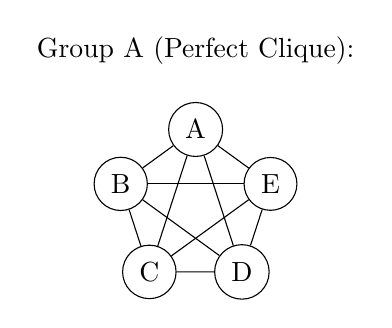
\begin{tikzpicture}
    \node at (0,2) {Group A (Perfect Clique):};
    \node[circle,draw] (A) at (90:1) {A};
    \node[circle,draw] (B) at (162:1) {B};
    \node[circle,draw] (C) at (234:1) {C};
    \node[circle,draw] (D) at (306:1) {D};
    \node[circle,draw] (E) at (18:1) {E};
    \draw (A) -- (B) -- (C) -- (D) -- (E) -- (A);
    \draw (A) -- (C);
    \draw (A) -- (D);
    \draw (B) -- (D);
    \draw (B) -- (E);
    \draw (C) -- (E);
\end{tikzpicture}
\hspace{1cm}
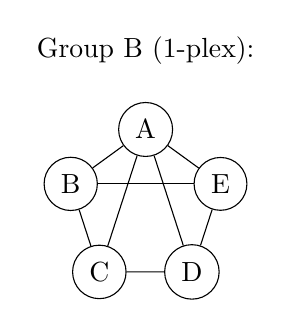
\begin{tikzpicture}
    \node at (0,2) {Group B (1-plex):};
    \node[circle,draw] (A) at (90:1) {A};
    \node[circle,draw] (B) at (162:1) {B};
    \node[circle,draw] (C) at (234:1) {C};
    \node[circle,draw] (D) at (306:1) {D};
    \node[circle,draw] (E) at (18:1) {E};
    \draw (A) -- (B) -- (C) -- (D) -- (E) -- (A);
    \draw (A) -- (C);
    \draw (A) -- (D);
    \draw (B) -- (E);
\end{tikzpicture}
\end{center}

\begin{enumerate}
    \item How many friends does each student have in Group A? \underline{\hspace{2cm}}
    \item In Group B, how many students is each person not friends with?

    \underline{\hspace{\textwidth}}
    \item Which group represents a perfect clique? \underline{\hspace{2cm}}
    \item Group B is called a 1-plex. Based on your observations, what do you think defines a k-plex?

    \underline{\hspace{\textwidth}}
\end{enumerate}

\subsection{Core Friends (k-core)}

Compare these two groups of 6 students:

\begin{center}
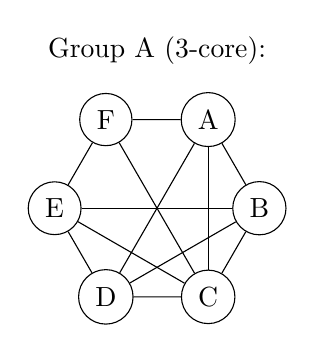
\begin{tikzpicture}
    \node at (0,2) {Group A (3-core):};
    \node[circle,draw] (A) at (60:1.3) {A};
    \node[circle,draw] (B) at (0:1.3) {B};
    \node[circle,draw] (C) at (300:1.3) {C};
    \node[circle,draw] (D) at (240:1.3) {D};
    \node[circle,draw] (E) at (180:1.3) {E};
    \node[circle,draw] (F) at (120:1.3) {F};
    \draw (A) -- (B) -- (C) -- (D) -- (E) -- (F) -- (A);
    \draw (A) -- (C);
    \draw (A) -- (D);
    \draw (B) -- (D);
    \draw (B) -- (E);
    \draw (C) -- (E);
    \draw (C) -- (F);
\end{tikzpicture}
\hspace{1cm}
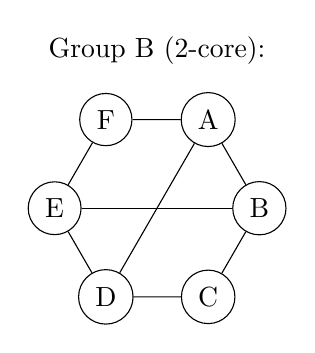
\begin{tikzpicture}
    \node at (0,2) {Group B (2-core):};
    \node[circle,draw] (A) at (60:1.3) {A};
    \node[circle,draw] (B) at (0:1.3) {B};
    \node[circle,draw] (C) at (300:1.3) {C};
    \node[circle,draw] (D) at (240:1.3) {D};
    \node[circle,draw] (E) at (180:1.3) {E};
    \node[circle,draw] (F) at (120:1.3) {F};
    \draw (A) -- (B) -- (C) -- (D) -- (E) -- (F) -- (A);
    \draw (A) -- (D);
    \draw (B) -- (E);
\end{tikzpicture}
\end{center}

\begin{enumerate}[resume]
    \item What's the minimum number of friends any student has in Group A? \underline{\hspace{2cm}}
    \item What's the minimum number of friends any student has in Group B? \underline{\hspace{2cm}}
    \item Group A is called a 3-core, and Group B is a 2-core. Based on your observations, what defines a k-core?

    \underline{\hspace{\textwidth}}
\end{enumerate}

\subsection{Density Matters ($\rho$-dense subgraphs)}

Compare these two groups of 5 students:

\begin{center}
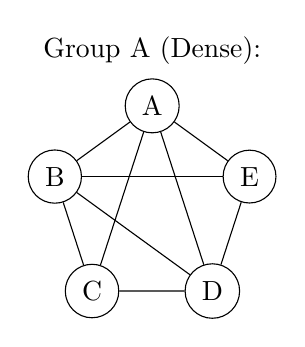
\begin{tikzpicture}
    \node at (0,2) {Group A (Dense):};
    \node[circle,draw] (A) at (90:1.3) {A};
    \node[circle,draw] (B) at (162:1.3) {B};
    \node[circle,draw] (C) at (234:1.3) {C};
    \node[circle,draw] (D) at (306:1.3) {D};
    \node[circle,draw] (E) at (18:1.3) {E};
    \draw (A) -- (B) -- (C) -- (D) -- (E) -- (A);
    \draw (A) -- (C);
    \draw (A) -- (D);
    \draw (B) -- (D);
    \draw (B) -- (E);
\end{tikzpicture}
\hspace{1cm}
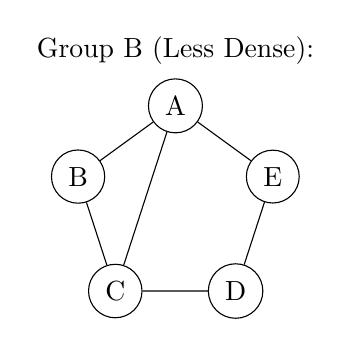
\begin{tikzpicture}
    \node at (0,2) {Group B (Less Dense):};
    \node[circle,draw] (A) at (90:1.3) {A};
    \node[circle,draw] (B) at (162:1.3) {B};
    \node[circle,draw] (C) at (234:1.3) {C};
    \node[circle,draw] (D) at (306:1.3) {D};
    \node[circle,draw] (E) at (18:1.3) {E};
    \draw (A) -- (B) -- (C) -- (D) -- (E) -- (A);
    \draw (A) -- (C);
\end{tikzpicture}
\end{center}

\begin{enumerate}[resume]
    \item How many total friendships are there in Group A? \underline{\hspace{2cm}}
    \item How many total friendships are there in Group B? \underline{\hspace{2cm}}
    \item Calculate the density for each group using this formula: density = (number of edges) / (maximum possible edges)

    Group A density: \underline{\hspace{2cm}} Group B density: \underline{\hspace{2cm}}
\end{enumerate}

\subsection{Extended Connections (n-clique)}

Compare these two groups of 6 students:

\begin{center}
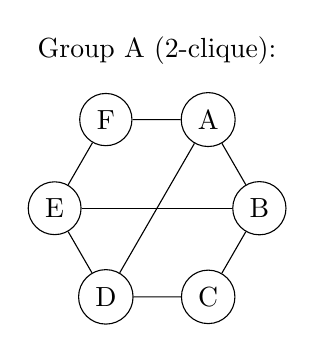
\begin{tikzpicture}
    \node at (0,2) {Group A (2-clique):};
    \node[circle,draw] (A) at (60:1.3) {A};
    \node[circle,draw] (B) at (0:1.3) {B};
    \node[circle,draw] (C) at (300:1.3) {C};
    \node[circle,draw] (D) at (240:1.3) {D};
    \node[circle,draw] (E) at (180:1.3) {E};
    \node[circle,draw] (F) at (120:1.3) {F};
    \draw (A) -- (B) -- (C) -- (D) -- (E) -- (F) -- (A);
    \draw (A) -- (D);
    \draw (B) -- (E);
\end{tikzpicture}
\hspace{1cm}
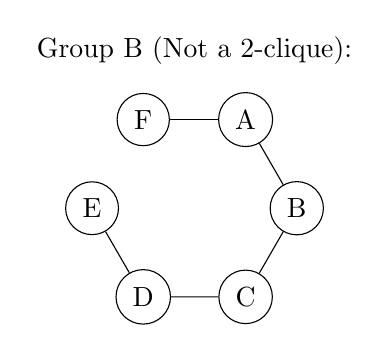
\begin{tikzpicture}
    \node at (0,2) {Group B (Not a 2-clique):};
    \node[circle,draw] (A) at (60:1.3) {A};
    \node[circle,draw] (B) at (0:1.3) {B};
    \node[circle,draw] (C) at (300:1.3) {C};
    \node[circle,draw] (D) at (240:1.3) {D};
    \node[circle,draw] (E) at (180:1.3) {E};
    \node[circle,draw] (F) at (120:1.3) {F};
    \draw (A) -- (B) -- (C) -- (D) -- (E);
    \draw (F) -- (A);
\end{tikzpicture}
\end{center}

\begin{enumerate}[resume]
    \item In Group A, what's the maximum distance from any student to any other? \underline{\hspace{2cm}}
    \item In Group B, what's the maximum distance from any student to any other? \underline{\hspace{2cm}}
    \item Group A is called a 2-clique. Based on your observations, what do you think defines an n-clique?
\end{enumerate}

\subsection{Triangles (k-truss)}

Compare these two groups of 6 students:

\begin{center}
    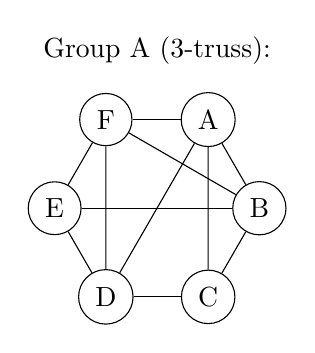
\begin{tikzpicture}
    \node at (0,2) {Group A (3-truss):};
    \node[circle,draw] (A) at (60:1.3) {A};
    \node[circle,draw] (B) at (0:1.3) {B};
    \node[circle,draw] (C) at (300:1.3) {C};
    \node[circle,draw] (D) at (240:1.3) {D};
    \node[circle,draw] (E) at (180:1.3) {E};
    \node[circle,draw] (F) at (120:1.3) {F};
    \draw (A) -- (B) -- (C) -- (A);
    \draw (D) -- (E) -- (F) -- (D);
    \draw (A) -- (D);
    \draw (B) -- (E);
    \draw (B) -- (F);
    \draw (F) -- (A);
    \draw (C) -- (D);
\end{tikzpicture}
\hspace{1cm}
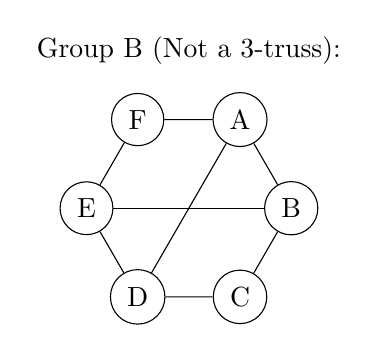
\begin{tikzpicture}
    \node at (0,2) {Group B (Not a 3-truss):};
    \node[circle,draw] (A) at (60:1.3) {A};
    \node[circle,draw] (B) at (0:1.3) {B};
    \node[circle,draw] (C) at (300:1.3) {C};
    \node[circle,draw] (D) at (240:1.3) {D};
    \node[circle,draw] (E) at (180:1.3) {E};
    \node[circle,draw] (F) at (120:1.3) {F};
    \draw (A) -- (B) -- (C) -- (D) -- (E) -- (F) -- (A);
    \draw (A) -- (D);
    \draw (B) -- (E);
\end{tikzpicture}
\end{center}

\begin{enumerate}[resume]
    \item In Group A, how many triangles (groups of 3 mutually connected friends) does each edge participate in? \underline{\hspace{2cm}}
    \begin{enumerate}
        \item A-B: \underline{\hspace{2cm}}
        \item B-C: \underline{\hspace{2cm}}
        \item C-D: \underline{\hspace{2cm}}
        \item D-E: \underline{\hspace{2cm}}
        \item E-F: \underline{\hspace{2cm}}
        \item F-A: \underline{\hspace{2cm}}
        \item A-C: \underline{\hspace{2cm}}
        \item A-D: \underline{\hspace{2cm}}
        \item B-E: \underline{\hspace{2cm}}
        \item B-F: \underline{\hspace{2cm}}
        \item D-F: \underline{\hspace{2cm}}
    \end{enumerate}
    \item In Group B, do all edges participate in at least one triangle? \underline{\hspace{2cm}}
    \item Group A is called a 3-truss. Based on your observations, what do you think defines a k-truss?
    \item How might the k-truss be related to the $k$-core?
\end{enumerate}

\section{Partitioning}

You will be given a network and asked to partition it into two communities. Answer the following questions for each network.

\subsection{Graph Cut}

Consider this network of 8 students:

\begin{center}
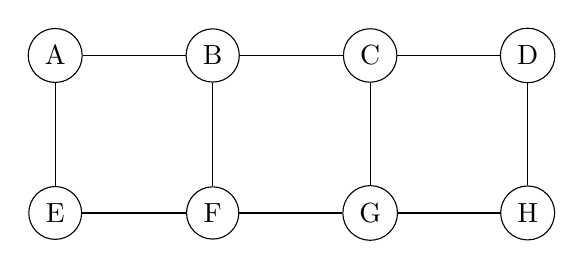
\begin{tikzpicture}
    \node[circle,draw] (A) at (0,2) {A};
    \node[circle,draw] (B) at (2,2) {B};
    \node[circle,draw] (C) at (4,2) {C};
    \node[circle,draw] (D) at (6,2) {D};
    \node[circle,draw] (E) at (0,0) {E};
    \node[circle,draw] (F) at (2,0) {F};
    \node[circle,draw] (G) at (4,0) {G};
    \node[circle,draw] (H) at (6,0) {H};
    \draw (A) -- (B) -- (C) -- (D);
    \draw (E) -- (F) -- (G) -- (H);
    \draw (A) -- (E);
    \draw (B) -- (F);
    \draw (C) -- (G);
    \draw (D) -- (H);
\end{tikzpicture}
\end{center}

\begin{enumerate}
    \item Draw a line to divide this network into two disconnected components. Explain why you chose to cut where you did. \textbf{Explanation: } \\ \ \\
    \underline{\hspace{\textwidth}}

    \item How many edges does your cut cross? \underline{\hspace{2cm}}

    \item This number of crossed edges is called the ``cut size''. What might be a problem with always choosing the cut that gives the smallest cut size?

    \underline{\hspace{\textwidth}}

\end{enumerate}

\clearpage
\subsection{Balanced Cut}

\begin{center}
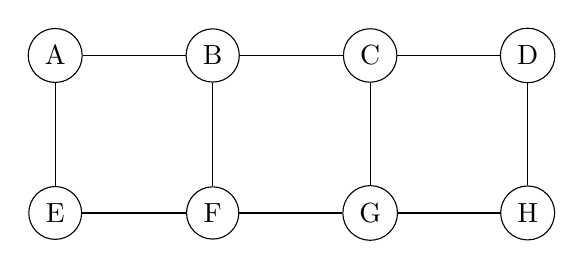
\begin{tikzpicture}
    \node[circle,draw] (A) at (0,2) {A};
    \node[circle,draw] (B) at (2,2) {B};
    \node[circle,draw] (C) at (4,2) {C};
    \node[circle,draw] (D) at (6,2) {D};
    \node[circle,draw] (E) at (0,0) {E};
    \node[circle,draw] (F) at (2,0) {F};
    \node[circle,draw] (G) at (4,0) {G};
    \node[circle,draw] (H) at (6,0) {H};
    \draw (A) -- (B) -- (C) -- (D);
    \draw (E) -- (F) -- (G) -- (H);
    \draw (A) -- (E);
    \draw (B) -- (F);
    \draw (C) -- (G);
    \draw (D) -- (H);
\end{tikzpicture}
\end{center}

\begin{enumerate}[resume]
    \item We want to balance the size of each community. The ``size'' of a community can be measured by the number of nodes it has, or the number of edges it has. The Ratio Cut does this by dividing the cut size by the number of nodes in each community:

    $$
    \text{Ratio Cut} = \text{cut size} * \left(\frac{1}{|A|} + \frac{1}{|B|}\right),
    $$

    where |A| and |B| are the number of nodes in each community. Find a cut that minimizes the Ratio Cut.

    \vspace{3cm}
    \item Normalized Cut instead uses the total degree (number of edges) of nodes in each community:

    $$
    \text{Normalized Cut} = \text{cut size} * \left(\frac{1}{\text{vol}(A)} + \frac{1}{\text{vol}(B)}\right),
    $$

    where vol(A) and vol(B) are the sum of the degrees of nodes in each community.

    Calculate the Normalized Cut for the same division.

    Normalized Cut = \underline{\hspace{4cm}}

    \vspace{3cm}
\end{enumerate}

\end{document}